
\section{Спиновый и орбитальный магнитные моменты атомов. Влияние кристаллического поля на магнетизм атомов. Магнитные моменты атомов переходных и редкоземельных элементов}


Рассмотрим электрон, который движется по окружности.
Поле, которое создаёт этот электрон выглядит как поле диполя. Такая система аналогична витку с током, где сила тока равна заряду, делённому на период вращения: $I =\frac{eV}{2\pi r}$.

\begin{figure}[h!]
    \centering
    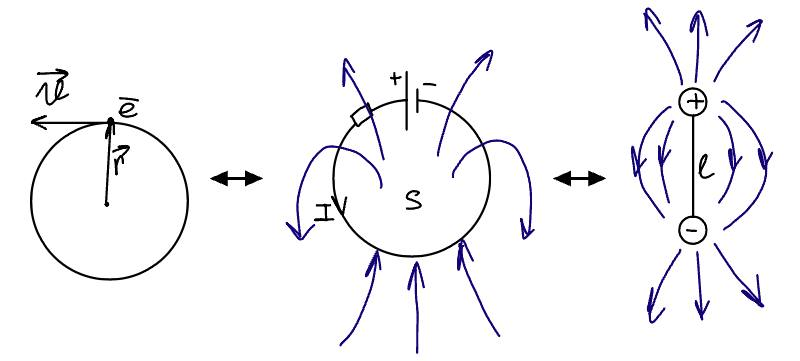
\includegraphics[width=0.6\textwidth]{ph23.1.jpg}
\end{figure}

Формула дипольного момента кольца с током: 
$\vec{m}=\frac{I \vec{S}}{c}$
($\quad\vec{m}$-- величина дипольного момента)


Согласно классической электродинамике, магнитный момент m кольца с током, охватывающего площадь S, равен (в системе СГС): 
$$
\vec{m}=\frac{1}{c}\left(\pi  r^2\right)  \frac{V}{2 \pi r} e=\frac{e}{2 c} V r  \frac{m_e}{m_e}=L  \frac{E}{2 c m_e}
$$

\textbf{$\Vec{L}$ – oрбитальный момент} количества движения электрона. Если учесть, что орбитальный (механический) момент электрона может принимать лишь дискретные значения, кратные постоянной Планка, то и значения магнитного момента электрона m могут быть только дискретными и магнитный момент электрона кратен магнетону Бора. Следовательно, $\mu_B$ играет роль элементарного магнитного момента --- <<кванта>> магнитного момента электрона.

$$
\begin{gathered}
\vec{m}=L * \frac{E}{2 c m_e} \\
\vec{L} \Longrightarrow\left\{\begin{array}{c}
|\vec{L}|=\hbar \sqrt{L(L+1)} \\
L_z=\hbar(L, \quad L-1, L-2, \quad \ldots-L) \\
\frac{e \hbar}{2 m_e c} \sqrt{L(L+1)}
\end{array}\right. \\
\vec{m} \Longrightarrow \frac{e \hbar}{2 m_e c}(L, L-1, L-2, \ldots-L) \\
\mu_B=\frac{e \hbar}{2 m_e c} \\
\mu_B=\frac{e \hbar}{2 m_e c} \approx 10^{-20}[\mathrm{emu}] \\
\mu_B=0,927 * 10^{-20} \mathrm{emu}[\mathrm{CГC}] \\
\mu_B=0,927 * 10^{-23} \frac{\text { Дж }}{\text { Тл }}[\mathrm{CH}]
\end{gathered}
$$


Схема возможных ориентаций орбитального момента:
\begin{figure}[h!]
    \centering
    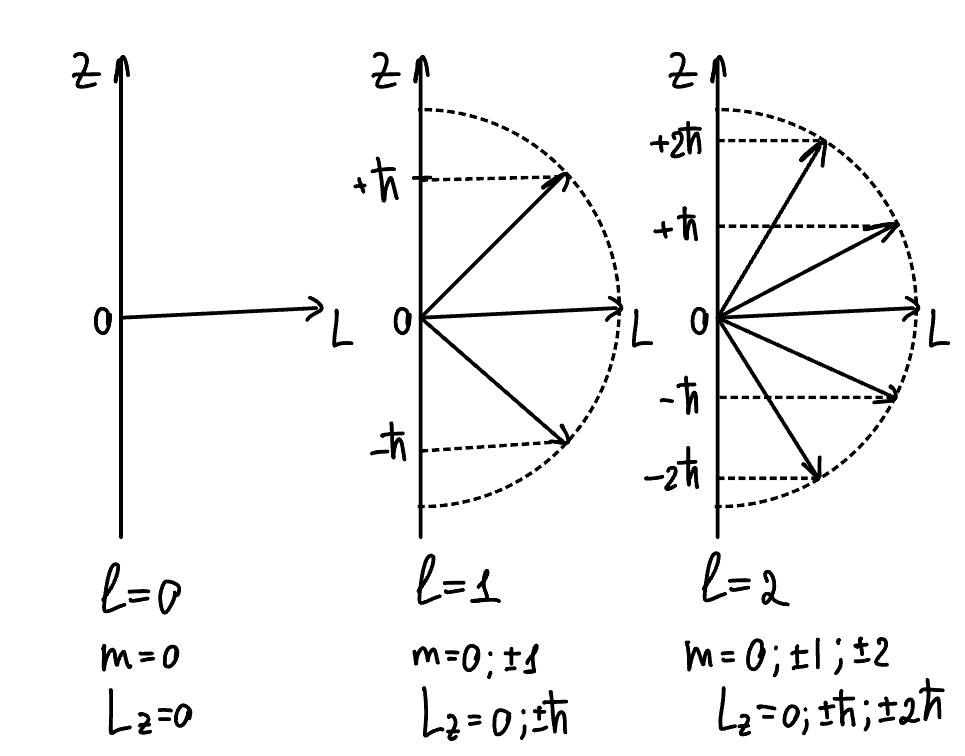
\includegraphics[width=0.8\textwidth]{ph23.3.jpg}
\end{figure}

\textbf{Спиновый магнитный момент} $\Vec{S}$ 
Полный магнитный момент $\Vec{J}$ электрона равен сумме векторов орбитального магнитного момента электрона и спинового магнитного момента.
(Нас интересует только та часть магнитного момента, которая сонаправлена с вектором J.)

\begin{figure}[h!]
    \centering
    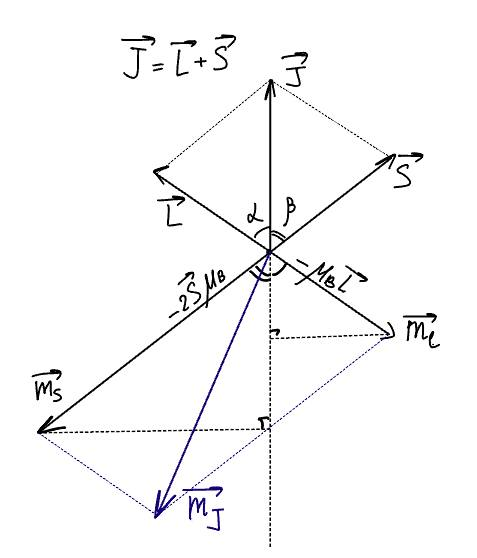
\includegraphics[width=0.6\textwidth]{ph23.2.jpg}
\end{figure}
$$
m_J=\mu_B|\vec{L}| * \cos \alpha+2 \mu_B|\vec{S}| * \cos \beta
$$
по теореме косинусов:
$$
\begin{aligned}
&|\vec{S}|=|\vec{L}|^2+|\vec{J}|^2-2|\vec{L}||\vec{J}| \cos \alpha \\
& \Rightarrow \cos \alpha= \frac{|\vec{L}|^2+|\vec{J}|^2-|\vec{S}|^2}{2|\vec{L}||\vec{J}|} \\
& \Rightarrow \cos \beta=\frac{-|\vec{L}|^2+|\vec{J}|^2+|\vec{S}|^2}{2|\vec{L}||\vec{J}|}
\end{aligned}
$$
$$
\begin{aligned}
& m_J=\mu_B\left(\frac{|\vec{L}|^2+|\vec{J}|^2+|\vec{S}|^2}{2|\vec{J}|}+2 \frac{-|\vec{L}|^2+|\vec{J}|^2+|\vec{S}|^2}{2|\vec{J}|}\right) * \frac{|\vec{J}|}{|\vec{J}|}=\mu_B\left(\frac{-|\vec{L}|^2+|\vec{J}|^2+|\vec{S}|^2}{2|\vec{J}|^2}\right)|\vec{J}| ; \\
& g=1+\frac{J(J+1)+S(S+1-L(L+1)}{2 J(J+1)} \\
& \left(\frac{-|\vec{L}|^2+|\vec{J}|^2+|\vec{S}|^2}{2|\vec{J}|^2}\right)-g-\text { фактор (фактор Ланде) } \\
& \text { T. e. } m_J=\mu_B  g |\vec{J}| \Rightarrow \vec{m}=\mu_B  g  \vec{J} \\
& \left\{\begin{array}{c}
|\vec{m}|=-\mu_B  g  \sqrt{J(J+1)} \\
m_z=\mu_B  g (J, J-1, \ldots-J)
\end{array}\right. \\
&
\end{aligned}
$$
3d-элементы проявляют чисто спиновый магнитный момент: L=0, $S\neq0$,  g=2

Это связано, с тем, что орбитальный момент заморожен в результате воздействия кристаллического поля.
d-металлы обладают большим радиусом d оболочки $\Rightarrow$ d-электроны не заэкранированы, следовательно, они подвергаются воздействию кристаллического поля: как бы «прикрепляются» к решётке. Таким образом, орбитальный момент «заморожен». Реализуется чисто спиновый механизм взаимодействия. 
\begin{figure}[h!]
    \centering
    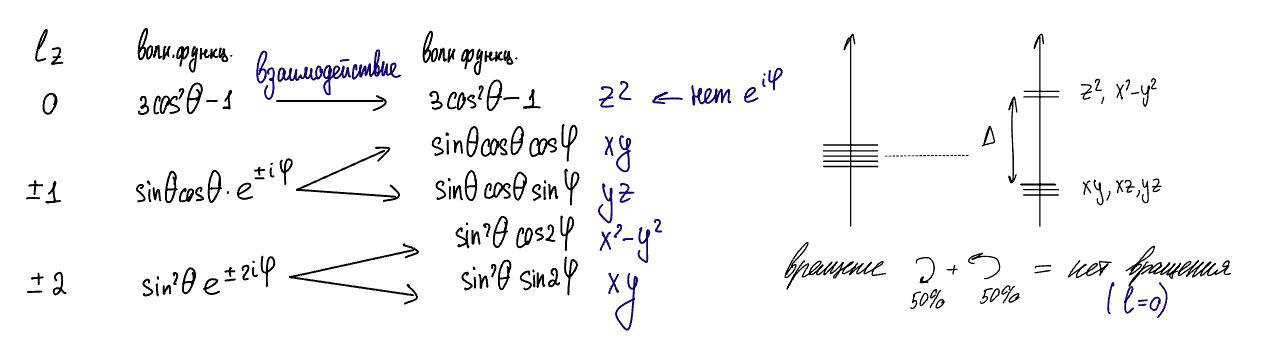
\includegraphics[width=1\textwidth]{ph23.4.jpg}
\end{figure}

РЗЭ --  4f электроны не взаимодействуют с кристаллическим полем, так как 4f электроны хорошо экранированы. $J=L+S$, $S\neq0$, $L\neq0$, 
$g=\frac{3}{2}+\frac{S(S+1)-L(L+1)}{2J(J+1)}$   (эта формула для g-фактора работает для всех РЗЭ, кроме Sm и Eu).


\section{Парамагнетизм. Функции Ланжевена и Бриллюэна. Закон Кюри-Вейсса.}

\textbf{Парамагнетики} --- вещества, которые намагничиваются во внешнем магнитном поле в направлении внешнего магнитного поля $ J \uparrow \uparrow H $ и имеют положительную магнитную восприимчивость $(\xi \ll 1)$, магнитная проницаемость незначительно отличается от 1  $ (\mu > \approx 1) $.


Рассмотрим классическую теорию парамагнетизма Ланжевена. Пусть имеется идеальный газ магнитных диполей с магнитными моментами $ \mu_0 $ и с концентрацией N. При этом взаимодействие между диполями явно не учитывается, но считается, что диполи участвуют в тепловом движении и при столкновениях направления магнитных моментов меняются. Если такой газ магнитных диполей находится в магнитном поле, то каждая диполь обладает потенциальной энергией: $U = - \mu_0 H \cos{(\theta)} $, где  $\theta$ -- угол между $ \mu_0 $ и H. 
\begin{figure}[h!]
    \centering
    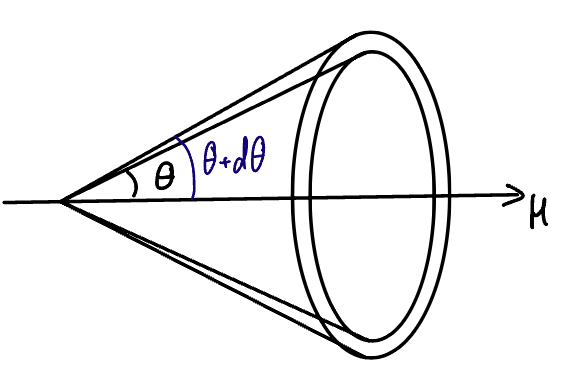
\includegraphics[width=0.4\textwidth]{ph24.1.jpg}
\end{figure}


Допустим, что для распределения диполей по энергии выполняется статистика Больцмана. Тогда вероятность того, что диполь направлен под углом $\theta$ к направлению поля пропорциональна: 
$e^{-\frac{U}{k T}}=e^{\frac{\mu_0 \mathrm{H} \cos \theta}{k T}}=e^{a \cos \theta}$, где $\mathrm{a}=\frac{\mu_0 \mathrm{H}} {\mathrm{kT}}$

Обозначим вероятность того, что диполь составляет с полем угол в интервале $\theta$ и $\theta + d \theta$, как $p(\theta)$. Для намагниченности М, т.е. магнитного момента единицы объема имеем: 
$$ \begin{aligned}
& M = \mu_0 N \int_0^\pi \cos{\theta p(\theta) d \theta} \\
& M=\mu_o N\left(\frac{e^a+e^{-a}}{e^a-e^{-a}}-\frac{1}{a}\right)=\mu_o N\left(\mathrm{coth} a-\frac{1}{a}\right)=\mu_o N L(a)
\end{aligned}
$$
\noindent где $L(a)$ - \textbf{функция Ланжевена}. 


При $a\rightarrow \infty$, что соответствует случаю, когда магнитная энергия много больше тепловой, $L(a)\rightarrow1 \text{ и } M=\mu_{0} N$, т.е. все диполи направлены по полю. При комнатной температуре такое условие реально не достижимо, так как при магнитном моменте в $\mu_B$ необходимо очень сильное поле (порядка $10^6$ Э, но при 1К $\frac{\mu_{В} N} {kT} \sim 1$ уже при  $10^4 $ Э)


При условии $a\ll 1$, L(а) можно разложить в ряд: 
$$ L(a)=\mathrm{coth} a-\frac{1}{a}=\frac{1}{a}+\frac{a}{3}-\frac{a^3}{45}+\ldots-\frac{1}{a} \approx \frac{a}{3} $$

Тогда для намагниченности получим: $ M = \frac{\mu_0 N a}{3} = \frac{\mu_0^2 N H }{3kT} $, и для восприимчивости имеем: $ \chi = \frac{\mu_0^2 N H }{3kT} = \frac{C}{T} $. Эта температурная зависимость называется \textbf{законом Кюри}, а коэффициент С – постоянной Кюри. 
\begin{figure}[h!]
    \centering
    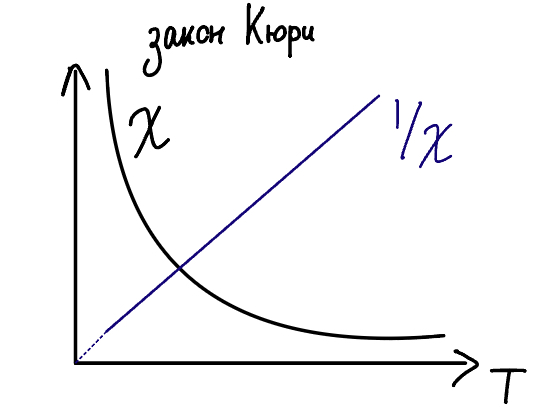
\includegraphics[width=0.4\textwidth]{ph24.2.jpg}
\end{figure}

Точка Кюри --- температура фазового перехода II рода, связанного со скачкообразным изменением свойств вещества. При температуре ниже точки Кюри ферромагнетики обладают спонтанной намагниченностью. Выше точки Кюри ферромагнетик оказывается разрушает его самопроизвольную намагниченность, в результате ферромагнетик становится парамагнетиком.


Так как на самом деле для магнитных атомов имеет место пространственное квантование, то необходимо рассматривать не непрерывное распределение магнитных диполей по направлению в пространстве, а возможные дискретные ориентации, определяемые условием пространственного квантования. Можно считать, что как и в классическом случае, справедливо статистическое распределение Больцмана.


Энергия атома в магнитном поле определяется теперь магнитными квантовыми числами $M_J$: $$U = - g_J \mu_B M_J H $$


Для вычисления намагниченности производится суммирование по всем возможным значениям $M_J$:
$$
\begin{aligned}
    & M=g_J \mu_B N \frac{\sum \limits_{M_J=-J}^{M_J=+J} M_J e^{\frac{g_{J} \mu_B M_J H}{k T}}}{\sum \limits_{M_J=-J}^{M_J=+J} e^{\frac{g_J \mu_B M_J H}{k T}}}=g_J \mu_B J N\left(\frac{2 J+1}{2 J} \mathrm{coth} \frac{2 J+1}{2 J} a-\frac{1}{2 J} \mathrm{coth} \frac{1}{2 J} a\right)= \\
    & =g_J \mu_B J N B_J(a)
\end{aligned}$$ 

\noindent где $a = \frac{g_J \mu_B J H}{kT}$, $\quad B_J(a)$ --- функция Бриллюэна.

В сильных полях и при низких температурах $a\rightarrow \infty, coth \rightarrow 1, B_J(a)\rightarrow 1$. Таким образом, при полном насыщении $M = g_J \mu_B J N $, то есть величина намагниченности отличается от полученной при классическом рассмотрении ($M=g_J \mu_B N \sqrt{J(J+1)}$).


При $a \ll 1$ функцию Бриллюэна можно разложить в ряд:
$$
B_J(a)=\frac{J+1}{3 J} a-\frac{\left[(J+1)^2+J^2\right](J+1)}{90 J^3} a^3+\ldots \ldots \ldots
$$
Оставив только первый член, то для восприимчивости получим: $$
\chi=\frac{\mathrm{g}_{\mathrm{J}}^2 \mu_{\mathrm{B}}^2 \mathrm{J}(\mathrm{J}+1) \mathrm{N}}{3 k T}
$$
что совпадает с выражением для восприимчивости при классическом рассмотрении.

Вейсс предположил, что на магнитный момент каждого атома действует некое
молекулярное поле $Н_{Е}$, пропорциональное намагниченности, т.е.
$$
H_E=\lambda M,
$$
где $\lambda$ - коэффициент молекулярного поля. Далее считается, что формула для
намагниченности в магнитном поле, полученная для невзаимодействующих
магнитных диполей, применима и в этом случае, но при учете того, что на
диполи действует не только внешнее, но и молекулярное поле  $Н_{Е}$. Тогда выражение для намагниченности примет вид:

$$
M=\mu_0 N L(a), \quad
a=\frac{\mu_0(H+\lambda M)}{k T}
 \Rightarrow
M=\frac{k T}{\mu_0 \lambda} a-\frac{H}{\lambda}
$$
Найдем теперь магнитную восприимчивость выше температуры Кюри:
$$
\chi=\frac{\partial M}{\partial H}=\mu_0 N L^{\prime}(a) \frac{\partial a}{\partial H}.
$$
$$
\frac{\partial a}{\partial H}=\frac{\mu_0}{k T}+\frac{\lambda \mu_0}{k T} \cdot \frac{\partial M}{\partial H}=\frac{\mu_0}{k T}+\frac{\lambda \mu_0}{k T} \chi.
$$
$$
\begin{aligned}
& \frac{\partial M}{\partial a}=\mu_0 N L^{\prime}(a) \approx \frac{1}{3} \mu_0 N, \\
& \frac{\partial M}{\partial a}=\frac{k T}{\lambda \mu_0}.
\end{aligned}
$$
(При высоких температурах $a \ll 1$ и в разложении $L(a)$ можно ограничиться первым членом $a / 3$ ) Тогда, получим
$$
\chi=\frac{\mu_0^2 N}{3 k\left(T-\frac{\mu_0^2 \lambda N}{3 k}\right)}
$$
Температура Кюри:
$$
T_C=\frac{\mu_0^2 \lambda N}{3 k}.
$$

$$
\chi=\frac{\mu_0^2 N}{3 k\left(T-T_C\right)}=\frac{C}{T-T_C}.
$$
Полученная зависимость --- \textbf{закон Кюри-Вейсса}. $C=\frac{\mu_0^2 N}{3 k}$ - постоянная Кюри.
\begin{figure}[h!]
\centering
    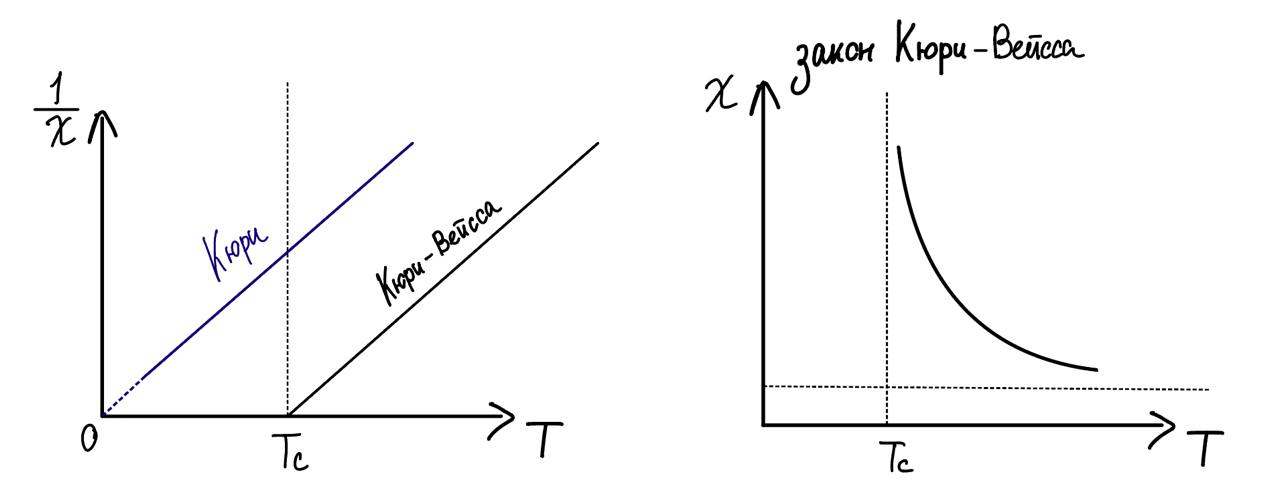
\includegraphics[width=0.8\textwidth]{ph24.3.jpg}
\end{figure}


\section{Парамагнетизм электронов проводимости}
Если рассматривать электроны проводимости в металлах в классическом представлении, как газ свободных частиц, то мы получили бы, что металлы должны обладать большой парамагнитной восприимчивостью, подчиняюшейся закону Кюри. На самом деле магнитная восприимчивость металлов не столь велика и слабо зависит от температуры, Объясняется это тем, что электроны проводимости в металле подчиняются статистике Ферми- Дирака, что кардинальным образом меняет подход к рассмотрению их магнитных свойств.
Плотность состояний свободных электронов в металле $\mathrm{G}$, как функция энергии электронов Е дается формулой
$$
G(E)=\frac{1}{2 \pi^2}\left(\frac{2 m}{\eta^2}\right)^{3 / 2} E^{1 / 2}
$$
Будем считать, что температура близка к $0 \mathrm{~K}$, все состояния с энергией меньше энергии Ферми $\mathrm{F}_{\mathrm{F}}$ заполнены и
$$
E_F=\frac{\eta^2}{2 m}\left(3 \pi^2 N\right)^{2 / 3}
$$
где $\mathrm{N}$ - число электронов в единице объема
\begin{figure}[h!]
    \centering
    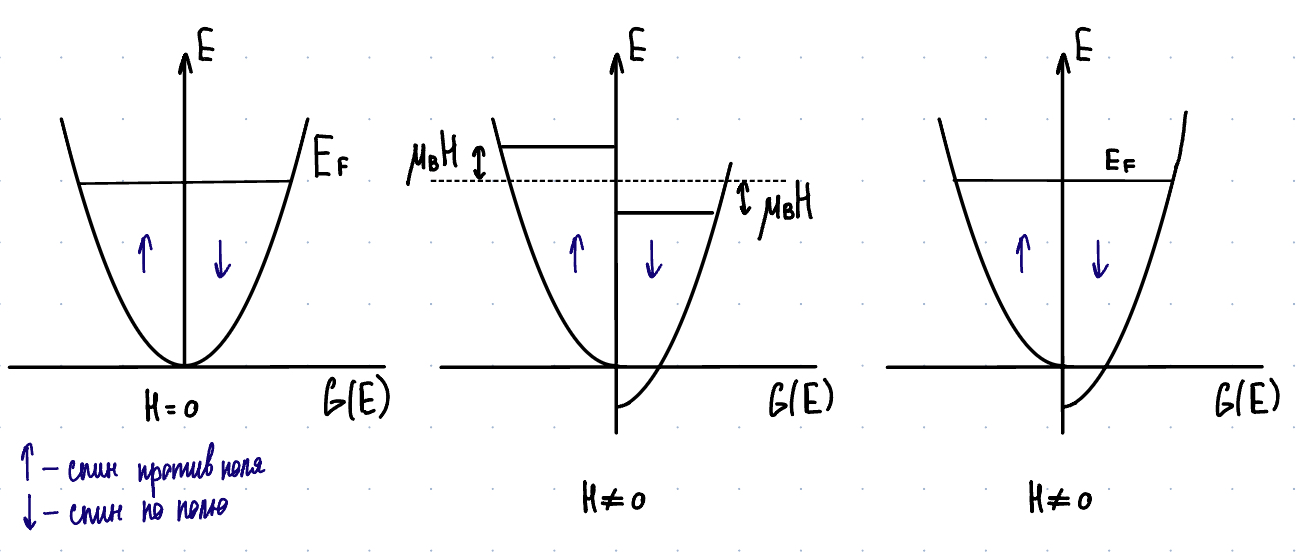
\includegraphics[width=1\textwidth]{ph25.1.jpg}
\end{figure}
При отсутствии поля сумма проекций спинов всех электронов на любую ось равна нулю и суммарная намагниченность равна нулю. При приложении поля у всех электронов со спином по полю энергия понизится на величину $\mu_{\mathrm{B}} \mathrm{H}$, а у электронов со спином против поля на такую же величину повысится. Так как уровень Ферми для всех электронов должен быть один и тот же, $ \frac{1}{2} G(E_F) \mu_{B} H$ 
(считаем $\mu_{\mathrm{B}} \mathrm{H}<<\mathrm{E}_{\mathrm{F}}$ ) электронов из левой части перейдет в правую  и таким образом электронов с магнитным моментом по полю станет больше на $\Delta \mathrm{n}$. Очевидно, что
$$
\Delta n=G\left(E_F\right) \mu_B H
$$
Тогда для намагниченности
$$
M=\mu_B \Delta n=G\left(E_F\right) \mu_B^2 H \quad
\Rightarrow \quad
M=\frac{3 \mu_B^2 N H}{2 E_F}
$$
Таким образом парамагнитная восприимчивость электронов проводимости в металле
$$
\chi_n^{\text{эл}}=\frac{3 \mu_B^2 N}{2 E_F}
$$
Как видно, $\chi_n^{\text{эл}}$ не зависит от температуры и значительно меньше по сравнению с восприимчивостью, если бы она следовала закону Кюри, так как в знаменателе вместо тепловой энергии кТ стоит величина на два-три порядка большая.

\section{Ферромагнетизм. Основные характеристики магнитного состояния ферромагнетика. Приближение молекулярного поля. Зонный ферромагнетизм. Доменная структура. Магнитный гистерезис.}
\textbf{Ферромагнетизм} – появление спонтанной намагниченности при температуре
ниже температуры Кюри вследствие упорядочения магнитных моментов, при котором
большая их часть параллельна друг другу. Вещества, в которых возникает ферромагнитное
упорядочение магнитных моментов, называются ферромагнетиками. Иными словами, ферромагнетик — такое вещество, которое
(при температуре ниже точки Кюри) способно обладать намагниченностью в отсутствии
внешнего магнитного поля.


Ферромагнитным материалам присуще явление \textbf{гистерезиса} – отставание изменения магнитной индукции В от изменения напряженности магнитного поля Н. Он обусловлен необратимыми изменениями энергетического состояния под действием внешнего поля Н. 
\begin{figure}[h!]
    \centering
    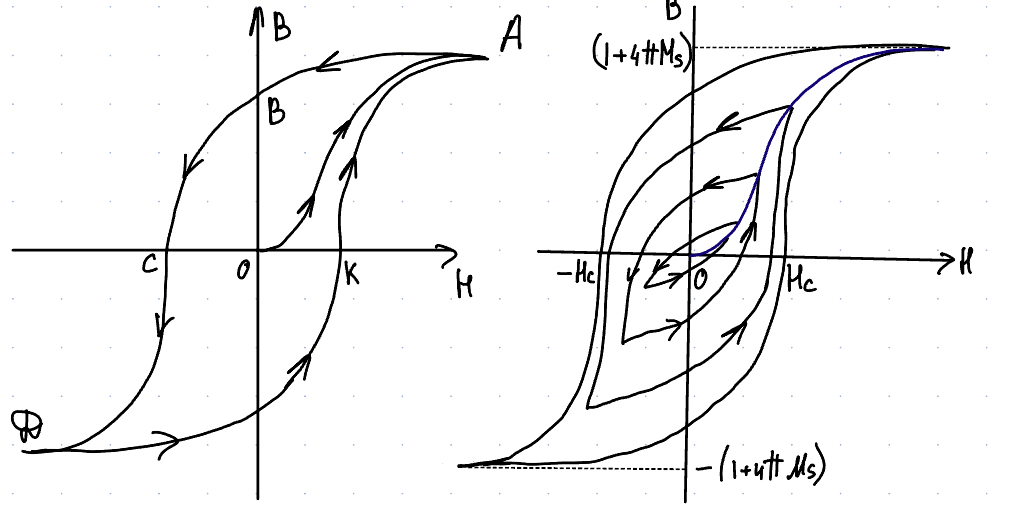
\includegraphics[width=0.8\textwidth]{ph26.1.jpg}
\end{figure}

Причины магнитного
гистерезиса : 1) задержки в движении доменных границ, обусловленные
дефектностью материала; 2) необратимые вращения намагниченности; 3) процессы
образования зародышей доменов с намагниченностью направленной более
благоприятно относительно направления поля.


При циклическом изменении поля от точки А индукция описывает
симметричную петлю гистерезиса АВСDКА. Отрезок ОВ соответствует остаточной
индукции (намагниченности), отрезок ОС – коэрцитивной силе. $H_C$ – коэерцитивная сила, это поле, которое нужно приложить к образцу, чтобы
размагнитить его остаточную намагниченность/ напряженность внешнего поля
необходимая для полного размагничивания образца.


Если снимать
симметричные петли гистерезиса при возрастающей амплитуде поля, то
вершины этих петель ложатся на кривую ОА, которая называется основной или
нормальной кривой намагничивания. Симметричная петля гистерезиса, в которой
достигается техническое насыщение, называется предельной петлей гистерезиса. Все
петли гистерезиса, лежащие внутри предельной петли, называются частными
петлями гистерезиса. 


\textbf{Приближение молекулярного поля ферромагнетиков}


Вейсс предположил, что на магнитный момент каждого атома действует некое молекулярное поле $ H_{E} $, пропорциональное намагниченности, т.е.
$$
H_E=\lambda M,
$$
где $\lambda$ - коэффициент молекулярного поля. Далее считается, что формула для
намагниченности в магнитном поле, полученная для невзаимодействующих
магнитных диполей, применима и в этом случае, но при учете того, что на
диполи действует не только внешнее, но и молекулярное поле $ H_{E} $. Тогда выражение для намагниченности примет вид:

$$
M=\mu_0 N L(a), \quad
a=\frac{\mu_0(H+\lambda M)}{k T}
 \Rightarrow
M=\frac{k T}{\mu_0 \lambda} a-\frac{H}{\lambda}
$$
Найдем теперь магнитную восприимчивость выше температуры Кюри:
$$
\chi=\frac{\partial M}{\partial H}=\mu_0 N L^{\prime}(a) \frac{\partial a}{\partial H}.
$$
$$
\frac{\partial a}{\partial H}=\frac{\mu_0}{k T}+\frac{\lambda \mu_0}{k T} \cdot \frac{\partial M}{\partial H}=\frac{\mu_0}{k T}+\frac{\lambda \mu_0}{k T} \chi.
$$
$$
\begin{aligned}
& \frac{\partial M}{\partial a}=\mu_0 N L^{\prime}(a) \approx \frac{1}{3} \mu_0 N, \\
& \frac{\partial M}{\partial a}=\frac{k T}{\lambda \mu_0}.
\end{aligned}
$$
(При высоких температурах $a<<1$ и в разложении L(a) можно ограничиться первым членом $a / 3$ ) Тогда, получим
$$
\chi=\frac{\mu_0^2 N}{3 k\left(T-\frac{\mu_0^2 \lambda N}{3 k}\right)}
$$
Температура Кюри:
$$
T_C=\frac{\mu_0^2 \lambda N}{3 k}.
$$

$$
\chi=\frac{\mu_0^2 N}{3 k\left(T-T_C\right)}=\frac{C}{T-T_C}.
$$
Полученная зависимость --- \textbf{закон Кюри-Вейсса} для магнитной восприимчивости ферромагнетика. $C=\frac{\mu_0^2 N}{3 k}$ - постоянная Кюри.
\begin{figure}[h!]
\centering
    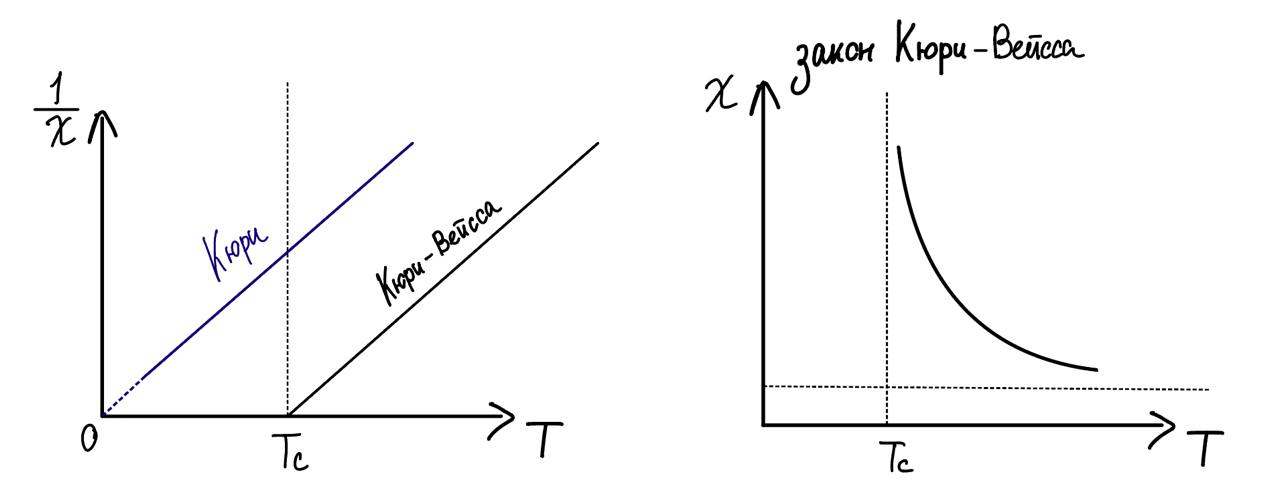
\includegraphics[width=0.8\textwidth]{ph24.3.jpg}
\end{figure}

\textbf{Зонный ферромагнитизм} --- магнетизм металлов и сплавов, интерпретируемый в рамках
моделей, основанных на зонной теории. Такие вещества называются зонными магнетиками; их типичные представители - переходные металлы (Fe, Со, Ni, Cr, Мn), их сплавы и соединения.Различают слабые и сильные зонные ферромагнетики. Слабыми называют зонные ферромагнетики, в которых спонтанное расщепление подзон меньше, чем энергетическая ширина зоны. Они характеризуются небольшим спонтанным моментом и стильной высокополевой восприимчивостью, связанной с тем, что с ростом поля продолжается перераспределение электронов между подзонами. В сильных ферромагнетиках все электроны находятся в одной подзоне и магнитная восприимчивость близка к нулю. В магнитное поле энергии электронов с противоположно ориентированными спинами различаются. Энергетическая зона разбивается на две подзоны, в одной из которых направление спинов совпадает с направлением приложенного поля, а в другой спиновые моменты ориентированы противоположно полю.


Плотность состояний свободных электронов в металле $\mathrm{G(E)}$ -- функция энергии электронов Е.

\begin{figure}[h!]
    \centering
    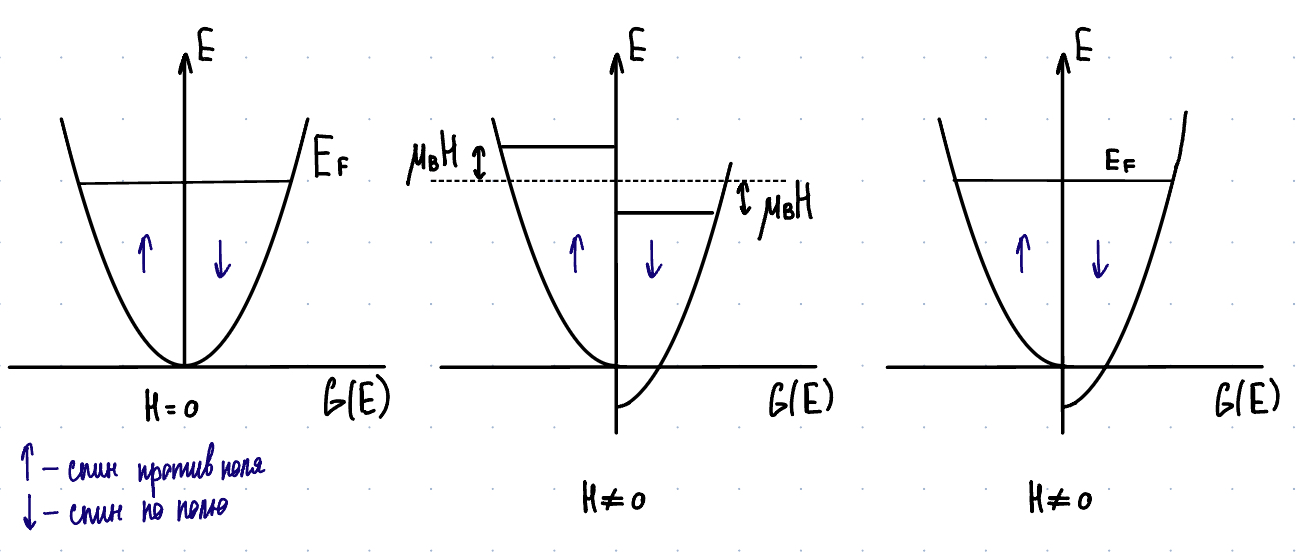
\includegraphics[width=1\textwidth]{ph25.1.jpg}
\end{figure}
 При приложении поля у всех электронов со спином по полю энергия понизится на величину $\mu_{\mathrm{B}} \mathrm{H}$, а у электронов со спином против поля на такую же величину повысится. Так как уровень Ферми для всех электронов должен быть один и тот же, $ \frac{1}{2} G(E_F) \mu_{B} H$ 
(считаем $\mu_{\mathrm{B}} \mathrm{H}<<\mathrm{E}_{\mathrm{F}}$ ) электронов из левой части перейдет в правую  и таким образом электронов с магнитным моментом по полю станет больше на $\Delta \mathrm{n}$. Очевидно, что
$$
\Delta n=G\left(E_F\right) \mu_B H
$$
Тогда для намагниченности
$$
M=G\left(E_F\right) \mu_B^2 H
$$
Таким образом парамагнитная восприимчивость
$$
\chi_p=G\left(E_F\right) \mu_B^2
$$
В системе невзаимодействуюших электронов фазовые переходы отсутствуют. Упет взапмодействия электронов приводнт к возникновению фазового перехода. Положите.тное обменное взаимодействие между электронами с обменным интегралом $I$ стремится выстроить все спины парадлельно, что влняет на магнитнуго воспрнимчивость парамагнетнка Паули:
$$
\chi_{\mathrm{exp}}=\frac{\chi_p}{1-\lambda \chi_p},
$$
где $\lambda=I / \mu_{\mathrm{B}}^2$ - параметр обменного взаимодействия. Из формулы (2.67) видно, что восприимчивость обменно-усиленного парамагнетнка возрастаст по мере возрастання $\lambda_{\chi_p}$. Прн выполнсннн устовня $\lambda \chi_0=1$ восприимчнвость стремнтся к бесконечностн, т. е. обменное взаимодействие приводит к самопронзвольному ферромагнитному упорндочснию. С учетом (2.66) условне возннкновсния ферромагнетнзма в снстеме коплективнзированных электронов с магнитнымн моментами $\mu_e=1 \mu_{\mathbb{B}}$, которое носит название критерня Стонера, имеет вид
$$
I G\left(E_{\mathrm{F}}\right) \geq 1
$$
\textbf{Доменная структура}
Магнитные моменты соседних атомов ферромагнетиков ориентированны параллельно,
однако в кристалле достаточно большой величины все магнитные моменты не могут быть
ориентированны параллельно. В противном случае вокруг кристалла появится магнитное
поле и энергия системы возрастет. Для снижения энергии системы кристалл разбивается на
домены - области спонтанной намагниченности, причем разбиение производится таким
образом, чтобы внешнее магнитное поле отсутствовало.
\begin{figure}[h!]
    \centering
    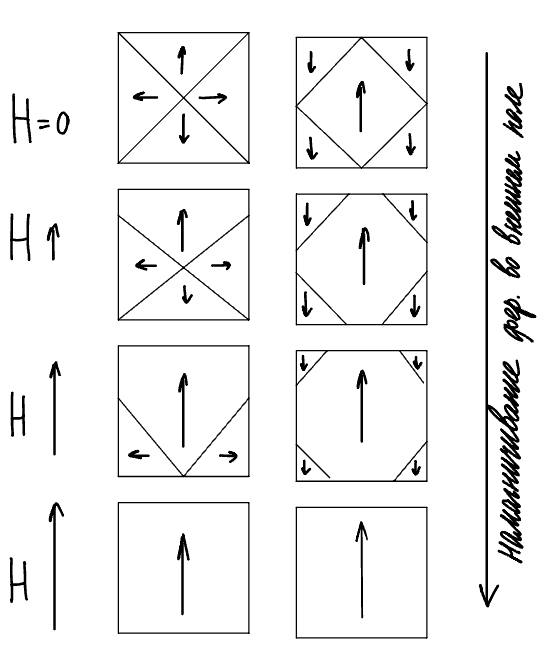
\includegraphics[width=0.4\textwidth]{ph26.2.jpg}
\end{figure}
При помещении ферромагнетика во внешнее магнитное поле векторы намагниченности
каких-либо доменов окажутся совпавшими или близкими к совпадению с вектором
напряжённости внешнего магнитного поля. Энергия таких доменов будет минимальной,
тогда как энергия всех остальных доменов повысится. Для того чтобы понизить энергию
системы благоприятно ориентированные домены растут. При этом увеличивается
намагниченность (М) и, следовательно, возрастает индукция (В).


На начальном участке кривой намагничивания увеличение напряженности внешнего поля ведет к незначительному росту индукции, причем при отключении внешнего поля индукция снижается до нуля. Этот участок принято называть участком обратимого намагничивания или областью Релея (I).

На втором участке незначительное изменение напряженности внешнего поля ведет к заметным изменениям индукции. Этот участок принято называть участком резкого роста индукции или областью скачков Баркгаузена (II).

На третьем участке кривой намагничивания зависимость индукции от напряженности внешнего поля вновь ослабевает. Этот участок называют участком замедленного намагничивания или область намагничивания за счет процессов вращения (III).

На четвертом участке индукция растет пропорционально напряженности магнитного поля. Этот участок называют участком насыщения или областью парапроцесса (IV).
\begin{figure}[h!]
    \centering
    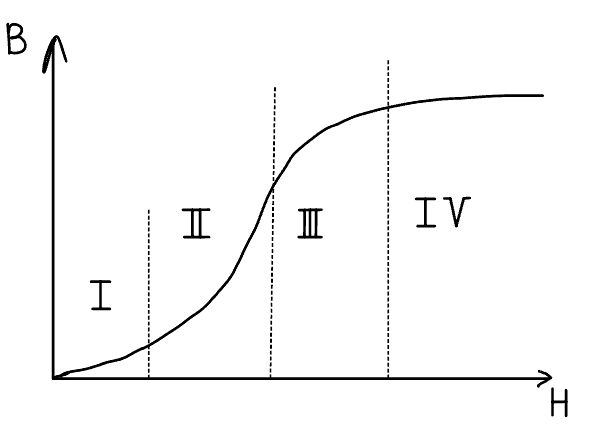
\includegraphics[width=0.4\textwidth]{ph26.3.jpg}
\end{figure}






\section{Природа магнетизма в твердых телах. Обменное взаимодействие. Типы магнитного упорядочения (ферромагнетизм, антиферромагнетизм, ферримагнетизм)}
В твердых телах с большим содержанием переходных элементов группы железа
или редких земель взаимодействие между атомами, обладающими магнитными
моментами, приводит к возникновению при температуре, характерной для каждого
вещества, магнитного упорядочения, т.е. наличию определенного дальнего порядка
в направлениях магнитных моментов атомов.
Причины происхождения магнитного момента атома:


\begin{enumerate}
    \item Спин электронов
    \item Орбитальный момент электронов связан с их вращением вокруг ядра
    \item Изменение орбитального момента при наложении внешнего магнитного поля.
\end{enumerate}


\textbf{ Обменное взаимодействие} --– квантовомеханический эффект, взаимодействие тождественных частиц, приводящее к зависимости значения энергии системы частиц от её полного спина. О.В. эффективно проявляется, когда «перекрываются» волновые функции отдельных частиц системы, т.е. когда существуют области пространства, в которых с заметной вероятностью может находиться частица в различных состояниях движения. 


Из принципа тождественности следует, что О.В. возникает в системе одинаковых частиц даже в случае, если прямыми силовыми взаимодействиями частиц можно пренебречь. Эффективно оно начинает проявляться, когда среднее расстояние между частицами сравнимо с длиной волны де Бройля, соответствующей средней скорости частиц.


Характер О.В. различен для фермионов и бозонов. Волновая функция бозонов (целый спин) – симметрична, а фермионов (полуцелый спин) – антисимметрична. Для фермионов О.В. – следствие принципа Паули, препятствующего сближению тождественных частиц с одинаковым направлением спинов. Оно проявляется в
отталкивании их друг от друга на расстояниях порядка или меньше длины волны де Бройля. В системе тождественных бозонов О.В. проявляется во взаимном притяжении частиц.


Пример О.В. для двухатомной молекулы:


$\Psi\left(\mathrm{r}_1, \mathrm{r}_2\right)=-\Psi\left(\mathrm{r}_2, \mathrm{r}_1\right)$ если спины параллельны (ФМ)


$\Psi\left(\mathrm{r}_1, \mathrm{r}_2\right)=\Psi\left(\mathrm{r}_2, \mathrm{r}_1\right)$ если спины антипараллельны (АФМ)


Если при разной взаимной ориентации спинов волновая функция разная, то $\mathrm{E}_{\uparrow \uparrow} \neq \mathrm{E}_{\uparrow \downarrow}$ $\mathrm{E}_{\uparrow \downarrow}^{\mathrm{T}}-$ синглет, $\mathrm{E}_{\uparrow \uparrow}^{\mathrm{S}}{- \text {триплет }}$
$$
\begin{gathered}
 \hat{\bar{S_1}} \text { и } \hat{\bar{S_2}}-\text { квантовые вектора } \\
 \hat{\bar{S}}= \hat{\bar{S_1}} +  \hat{\bar{S_2}} ; \quad S=\frac{1}{2}, \quad S-1 ; 0 \\
|\hat{\bar{S}}|^2=\left| \hat{\bar{S_1}}\right|^2+2\left( \hat{\bar{S_1}},  \hat{\bar{S_2}}\right)+\left| \hat{\bar{S_2}}\right|^2 \\
\mathrm{~S}(\mathrm{~S}+1)=2 \mathrm{~S}(\mathrm{~S}+1)+2\left( \hat{\bar{S_1}},  \hat{\bar{S_2}}\right) \\
\left( \hat{\bar{S_1}}, \hat{\bar{S_2}}\right)=\frac{S(S+1)}{2}-\frac{S}{4}
\end{gathered}
$$


Синглет: $\mathrm{S}=0,\left( \hat{\bar{S_1}}, \hat{\bar{S_2}}\right)=-\frac{3}{4}$


Триплет: $\mathrm{S}=1,\left( \hat{\bar{S_1}},  \hat{\bar{S_2}}\right)=\frac{1}{4}$
$$
\begin{aligned}
& E_{\uparrow \uparrow}=E_0+ \frac{1}{4} \mathrm{~J} \\
& E_{\uparrow \downarrow}=E_0- \frac{3}{4} \mathrm{~J}
\end{aligned}
$$


$\mathrm{J}=\mathrm{E}_{\uparrow \uparrow}-\mathrm{E}_{\uparrow \downarrow}-$ обменный интеграл


Базовая энергия: $E_0=\frac{3 E_{\uparrow \uparrow}+E_{\uparrow \downarrow}}{4}$


$\mathrm{E}=\mathrm{E}_0+J\left( \hat{\bar{S_1}}, \hat{\bar{S_2}}\right)-$ обмен Гейзенберга


\textbf{ Типы магнитного упорядочения:}
$$
\begin{array}{|l|l|l|l|}
\hline & \text { Знак } \chi & |\chi| & \mu \\
\hline \text { Диамагнетизм } & - & 10^{-8}-10^{-4} & <1 \\
\hline \text { Парамагнетизм } & + & 10^{-6}-10^{-3} & >1 \\
\hline \text { Ферромагнетизм } & +, \chi(\mathrm{H}) & 10^2-10^4 & \mu(\mathrm{H})>>1 \\
\hline \text { Антиферромагнетизм } & +, \chi(\mathrm{H}) & 10^{-4}-10^{-2} & \mu(\mathrm{H})>>1 \\
\hline \text { Ферримагнетизм } & +, \chi(\mathrm{H}) & 10^1-10^3 & >1 \\
\hline
\end{array}
$$
 (H - напряжённость магнитного поля, $\chi$ - магнитная восприимчивость, $\mu$ - магнитная проницаемость)
\begin{figure}[h!]
    \centering
    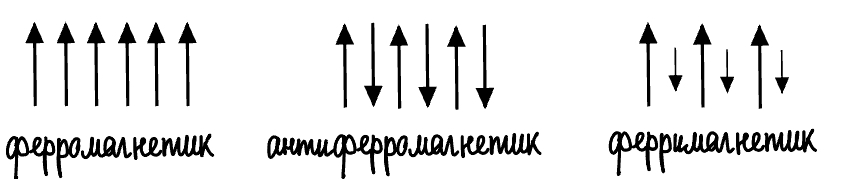
\includegraphics[width=0.8\textwidth]{ph27.1.jpg}
\end{figure}

\textbf{Ферромагнетик} – доменная структура у всех атомов одинаковый магнитный момент


\textbf{Антиферромагнетик} – магнитные моменты ориентированы антипараллельно 


\textbf{Ферримагнетик} – магнитные моменты соседних атомов ориентированы антипараллельно и имеют разную величину


\textbf{Парамагнетик} – векторы магнитных моментов разориентированы







